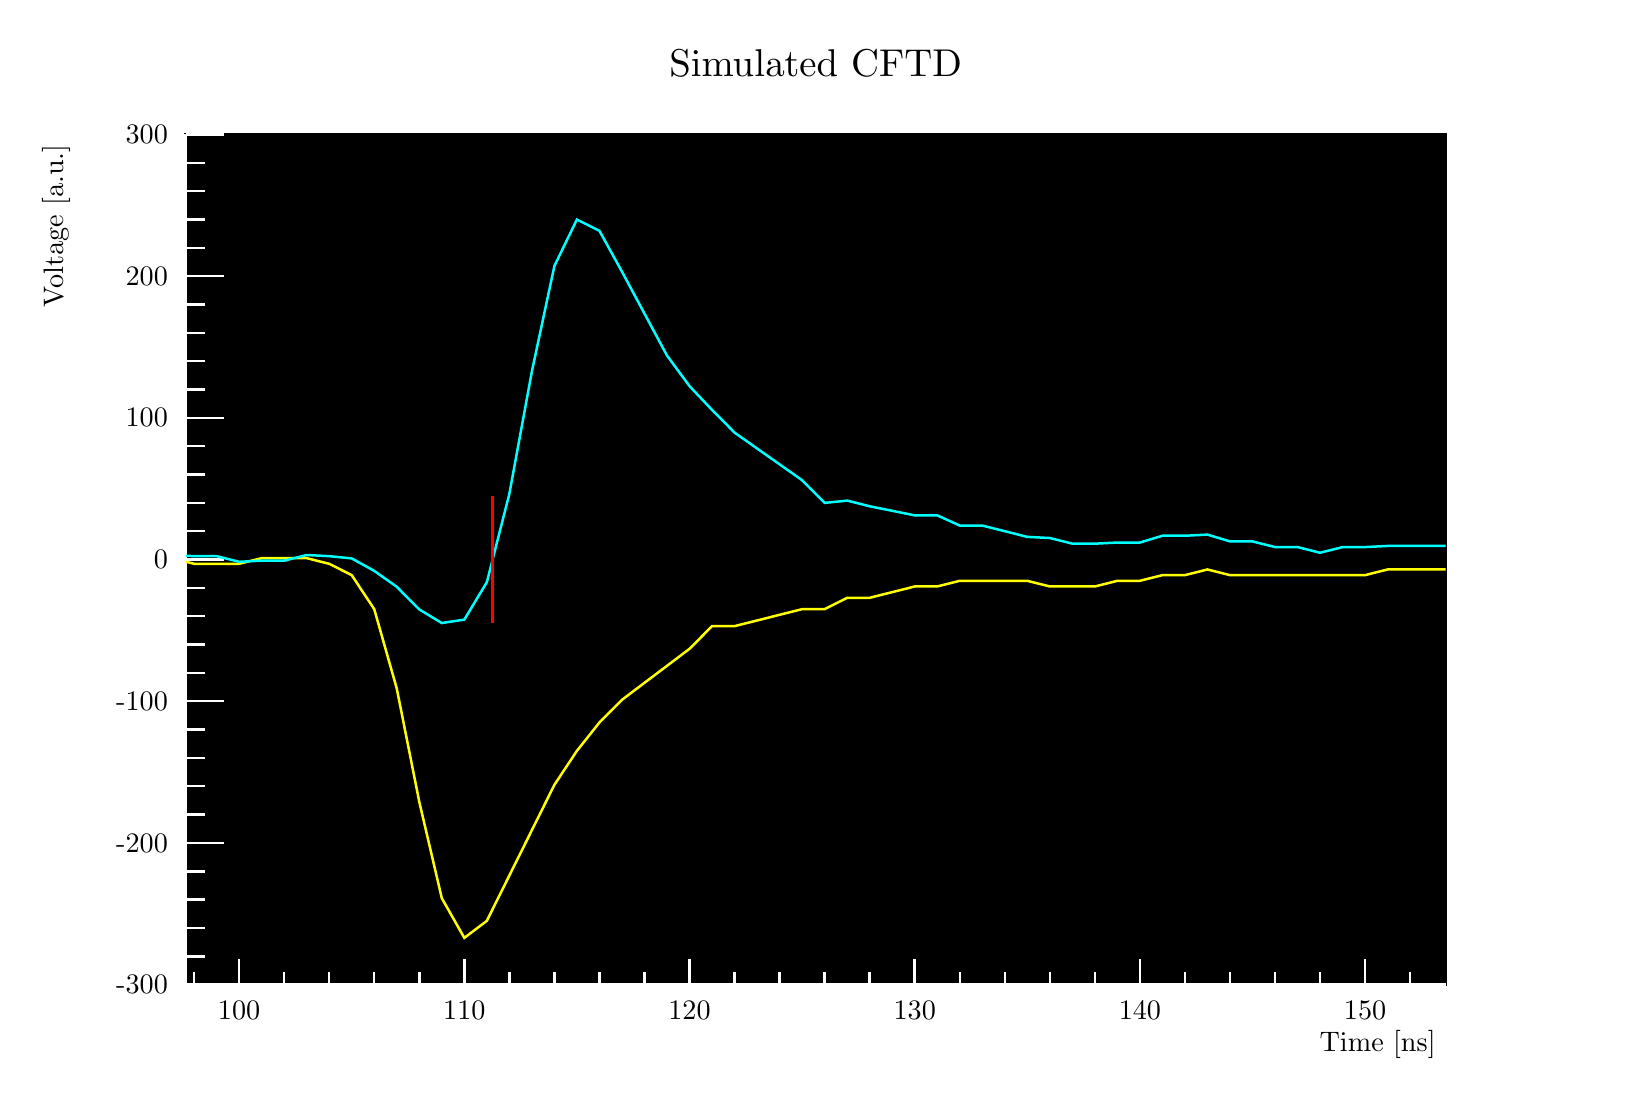
\begin{tikzpicture}
\pgfdeclareplotmark{cross} {
\pgfpathmoveto{\pgfpoint{-0.3\pgfplotmarksize}{\pgfplotmarksize}}
\pgfpathlineto{\pgfpoint{+0.3\pgfplotmarksize}{\pgfplotmarksize}}
\pgfpathlineto{\pgfpoint{+0.3\pgfplotmarksize}{0.3\pgfplotmarksize}}
\pgfpathlineto{\pgfpoint{+1\pgfplotmarksize}{0.3\pgfplotmarksize}}
\pgfpathlineto{\pgfpoint{+1\pgfplotmarksize}{-0.3\pgfplotmarksize}}
\pgfpathlineto{\pgfpoint{+0.3\pgfplotmarksize}{-0.3\pgfplotmarksize}}
\pgfpathlineto{\pgfpoint{+0.3\pgfplotmarksize}{-1.\pgfplotmarksize}}
\pgfpathlineto{\pgfpoint{-0.3\pgfplotmarksize}{-1.\pgfplotmarksize}}
\pgfpathlineto{\pgfpoint{-0.3\pgfplotmarksize}{-0.3\pgfplotmarksize}}
\pgfpathlineto{\pgfpoint{-1.\pgfplotmarksize}{-0.3\pgfplotmarksize}}
\pgfpathlineto{\pgfpoint{-1.\pgfplotmarksize}{0.3\pgfplotmarksize}}
\pgfpathlineto{\pgfpoint{-0.3\pgfplotmarksize}{0.3\pgfplotmarksize}}
\pgfpathclose
\pgfusepathqstroke
}
\pgfdeclareplotmark{cross*} {
\pgfpathmoveto{\pgfpoint{-0.3\pgfplotmarksize}{\pgfplotmarksize}}
\pgfpathlineto{\pgfpoint{+0.3\pgfplotmarksize}{\pgfplotmarksize}}
\pgfpathlineto{\pgfpoint{+0.3\pgfplotmarksize}{0.3\pgfplotmarksize}}
\pgfpathlineto{\pgfpoint{+1\pgfplotmarksize}{0.3\pgfplotmarksize}}
\pgfpathlineto{\pgfpoint{+1\pgfplotmarksize}{-0.3\pgfplotmarksize}}
\pgfpathlineto{\pgfpoint{+0.3\pgfplotmarksize}{-0.3\pgfplotmarksize}}
\pgfpathlineto{\pgfpoint{+0.3\pgfplotmarksize}{-1.\pgfplotmarksize}}
\pgfpathlineto{\pgfpoint{-0.3\pgfplotmarksize}{-1.\pgfplotmarksize}}
\pgfpathlineto{\pgfpoint{-0.3\pgfplotmarksize}{-0.3\pgfplotmarksize}}
\pgfpathlineto{\pgfpoint{-1.\pgfplotmarksize}{-0.3\pgfplotmarksize}}
\pgfpathlineto{\pgfpoint{-1.\pgfplotmarksize}{0.3\pgfplotmarksize}}
\pgfpathlineto{\pgfpoint{-0.3\pgfplotmarksize}{0.3\pgfplotmarksize}}
\pgfpathclose
\pgfusepathqfillstroke
}
\pgfdeclareplotmark{newstar} {
\pgfpathmoveto{\pgfqpoint{0pt}{\pgfplotmarksize}}
\pgfpathlineto{\pgfqpointpolar{44}{0.5\pgfplotmarksize}}
\pgfpathlineto{\pgfqpointpolar{18}{\pgfplotmarksize}}
\pgfpathlineto{\pgfqpointpolar{-20}{0.5\pgfplotmarksize}}
\pgfpathlineto{\pgfqpointpolar{-54}{\pgfplotmarksize}}
\pgfpathlineto{\pgfqpointpolar{-90}{0.5\pgfplotmarksize}}
\pgfpathlineto{\pgfqpointpolar{234}{\pgfplotmarksize}}
\pgfpathlineto{\pgfqpointpolar{198}{0.5\pgfplotmarksize}}
\pgfpathlineto{\pgfqpointpolar{162}{\pgfplotmarksize}}
\pgfpathlineto{\pgfqpointpolar{134}{0.5\pgfplotmarksize}}
\pgfpathclose
\pgfusepathqstroke
}
\pgfdeclareplotmark{newstar*} {
\pgfpathmoveto{\pgfqpoint{0pt}{\pgfplotmarksize}}
\pgfpathlineto{\pgfqpointpolar{44}{0.5\pgfplotmarksize}}
\pgfpathlineto{\pgfqpointpolar{18}{\pgfplotmarksize}}
\pgfpathlineto{\pgfqpointpolar{-20}{0.5\pgfplotmarksize}}
\pgfpathlineto{\pgfqpointpolar{-54}{\pgfplotmarksize}}
\pgfpathlineto{\pgfqpointpolar{-90}{0.5\pgfplotmarksize}}
\pgfpathlineto{\pgfqpointpolar{234}{\pgfplotmarksize}}
\pgfpathlineto{\pgfqpointpolar{198}{0.5\pgfplotmarksize}}
\pgfpathlineto{\pgfqpointpolar{162}{\pgfplotmarksize}}
\pgfpathlineto{\pgfqpointpolar{134}{0.5\pgfplotmarksize}}
\pgfpathclose
\pgfusepathqfillstroke
}
\definecolor{c}{rgb}{1,1,1};
\draw [color=c, fill=c] (0,0) rectangle (20,13.4957);
\definecolor{c}{rgb}{0,0,0};
\draw [color=c, fill=c] (2,1.34957) rectangle (18,12.1461);
\draw [c,line width=0.9] (2,1.34957) -- (2,12.1461) -- (18,12.1461) -- (18,1.34957) -- (2,1.34957);
\draw [color=c, fill=c] (2,1.34957) rectangle (18,12.1461);
\draw [c,line width=0.9] (2,1.34957) -- (2,12.1461) -- (18,12.1461) -- (18,1.34957) -- (2,1.34957);
\definecolor{c}{rgb}{1,1,1};
\draw [c,line width=0.9] (2,1.34957) -- (18,1.34957);
\draw [c,line width=0.9] (2.67838,1.67347) -- (2.67838,1.34957);
\draw [c,line width=0.9] (3.25037,1.51152) -- (3.25037,1.34957);
\draw [c,line width=0.9] (3.82237,1.51152) -- (3.82237,1.34957);
\draw [c,line width=0.9] (4.39437,1.51152) -- (4.39437,1.34957);
\draw [c,line width=0.9] (4.96637,1.51152) -- (4.96637,1.34957);
\draw [c,line width=0.9] (5.53837,1.67347) -- (5.53837,1.34957);
\draw [c,line width=0.9] (6.11037,1.51152) -- (6.11037,1.34957);
\draw [c,line width=0.9] (6.68237,1.51152) -- (6.68237,1.34957);
\draw [c,line width=0.9] (7.25437,1.51152) -- (7.25437,1.34957);
\draw [c,line width=0.9] (7.82636,1.51152) -- (7.82636,1.34957);
\draw [c,line width=0.9] (8.39836,1.67347) -- (8.39836,1.34957);
\draw [c,line width=0.9] (8.97036,1.51152) -- (8.97036,1.34957);
\draw [c,line width=0.9] (9.54236,1.51152) -- (9.54236,1.34957);
\draw [c,line width=0.9] (10.1144,1.51152) -- (10.1144,1.34957);
\draw [c,line width=0.9] (10.6864,1.51152) -- (10.6864,1.34957);
\draw [c,line width=0.9] (11.2584,1.67347) -- (11.2584,1.34957);
\draw [c,line width=0.9] (11.8304,1.51152) -- (11.8304,1.34957);
\draw [c,line width=0.9] (12.4024,1.51152) -- (12.4024,1.34957);
\draw [c,line width=0.9] (12.9744,1.51152) -- (12.9744,1.34957);
\draw [c,line width=0.9] (13.5464,1.51152) -- (13.5464,1.34957);
\draw [c,line width=0.9] (14.1184,1.67347) -- (14.1184,1.34957);
\draw [c,line width=0.9] (14.6904,1.51152) -- (14.6904,1.34957);
\draw [c,line width=0.9] (15.2624,1.51152) -- (15.2624,1.34957);
\draw [c,line width=0.9] (15.8343,1.51152) -- (15.8343,1.34957);
\draw [c,line width=0.9] (16.4063,1.51152) -- (16.4063,1.34957);
\draw [c,line width=0.9] (16.9783,1.67347) -- (16.9783,1.34957);
\draw [c,line width=0.9] (2.67838,1.67347) -- (2.67838,1.34957);
\draw [c,line width=0.9] (2.10638,1.51152) -- (2.10638,1.34957);
\draw [c,line width=0.9] (16.9783,1.67347) -- (16.9783,1.34957);
\draw [c,line width=0.9] (17.5503,1.51152) -- (17.5503,1.34957);
\definecolor{c}{rgb}{0,0,0};
\draw [anchor=base] (2.67838,0.904212) node[scale=1.01821, color=c, rotate=0]{100};
\draw [anchor=base] (5.53837,0.904212) node[scale=1.01821, color=c, rotate=0]{110};
\draw [anchor=base] (8.39836,0.904212) node[scale=1.01821, color=c, rotate=0]{120};
\draw [anchor=base] (11.2584,0.904212) node[scale=1.01821, color=c, rotate=0]{130};
\draw [anchor=base] (14.1184,0.904212) node[scale=1.01821, color=c, rotate=0]{140};
\draw [anchor=base] (16.9783,0.904212) node[scale=1.01821, color=c, rotate=0]{150};
\draw [anchor= east] (18,0.593811) node[scale=1.01821, color=c, rotate=0]{Time [ns]};
\definecolor{c}{rgb}{1,1,1};
\draw [c,line width=0.9] (2,1.34957) -- (2,12.1461);
\draw [c,line width=0.9] (2.48,1.34957) -- (2,1.34957);
\draw [c,line width=0.9] (2.24,1.70946) -- (2,1.70946);
\draw [c,line width=0.9] (2.24,2.06934) -- (2,2.06934);
\draw [c,line width=0.9] (2.24,2.42923) -- (2,2.42923);
\draw [c,line width=0.9] (2.24,2.78911) -- (2,2.78911);
\draw [c,line width=0.9] (2.48,3.149) -- (2,3.149);
\draw [c,line width=0.9] (2.24,3.50888) -- (2,3.50888);
\draw [c,line width=0.9] (2.24,3.86877) -- (2,3.86877);
\draw [c,line width=0.9] (2.24,4.22865) -- (2,4.22865);
\draw [c,line width=0.9] (2.24,4.58854) -- (2,4.58854);
\draw [c,line width=0.9] (2.48,4.94842) -- (2,4.94842);
\draw [c,line width=0.9] (2.24,5.30831) -- (2,5.30831);
\draw [c,line width=0.9] (2.24,5.66819) -- (2,5.66819);
\draw [c,line width=0.9] (2.24,6.02808) -- (2,6.02808);
\draw [c,line width=0.9] (2.24,6.38797) -- (2,6.38797);
\draw [c,line width=0.9] (2.48,6.74785) -- (2,6.74785);
\draw [c,line width=0.9] (2.24,7.10774) -- (2,7.10774);
\draw [c,line width=0.9] (2.24,7.46762) -- (2,7.46762);
\draw [c,line width=0.9] (2.24,7.82751) -- (2,7.82751);
\draw [c,line width=0.9] (2.24,8.18739) -- (2,8.18739);
\draw [c,line width=0.9] (2.48,8.54728) -- (2,8.54728);
\draw [c,line width=0.9] (2.24,8.90716) -- (2,8.90716);
\draw [c,line width=0.9] (2.24,9.26705) -- (2,9.26705);
\draw [c,line width=0.9] (2.24,9.62693) -- (2,9.62693);
\draw [c,line width=0.9] (2.24,9.98682) -- (2,9.98682);
\draw [c,line width=0.9] (2.48,10.3467) -- (2,10.3467);
\draw [c,line width=0.9] (2.24,10.7066) -- (2,10.7066);
\draw [c,line width=0.9] (2.24,11.0665) -- (2,11.0665);
\draw [c,line width=0.9] (2.24,11.4264) -- (2,11.4264);
\draw [c,line width=0.9] (2.24,11.7862) -- (2,11.7862);
\draw [c,line width=0.9] (2.48,12.1461) -- (2,12.1461);
\definecolor{c}{rgb}{0,0,0};
\draw [anchor= east] (1.9,1.34957) node[scale=1.01821, color=c, rotate=0]{-300};
\draw [anchor= east] (1.9,3.149) node[scale=1.01821, color=c, rotate=0]{-200};
\draw [anchor= east] (1.9,4.94842) node[scale=1.01821, color=c, rotate=0]{-100};
\draw [anchor= east] (1.9,6.74785) node[scale=1.01821, color=c, rotate=0]{0};
\draw [anchor= east] (1.9,8.54728) node[scale=1.01821, color=c, rotate=0]{100};
\draw [anchor= east] (1.9,10.3467) node[scale=1.01821, color=c, rotate=0]{200};
\draw [anchor= east] (1.9,12.1461) node[scale=1.01821, color=c, rotate=0]{300};
\draw [anchor= east] (0.354441,12.1461) node[scale=1.01821, color=c, rotate=90]{Voltage [a.u.]};
\definecolor{c}{rgb}{1,1,0};
\draw [c,line width=0.9] (2,6.72064) -- (2.10638,6.69387);
\draw [c,line width=0.9] (2.10638,6.69387) -- (2.39238,6.69387) -- (2.67838,6.69387) -- (2.96437,6.76585) -- (3.25037,6.76585) -- (3.53637,6.76585) -- (3.82237,6.69387) -- (4.10837,6.54991) -- (4.39437,6.11805) -- (4.68037,5.11037) --
 (4.96637,3.67083) -- (5.25237,2.44722) -- (5.53837,1.94338) -- (5.82437,2.15931) -- (6.11037,2.73513) -- (6.39637,3.31095) -- (6.68237,3.88676) -- (6.96837,4.31862) -- (7.25437,4.67851) -- (7.54037,4.96642) -- (7.82636,5.18235) -- (8.11236,5.39828)
 -- (8.39836,5.61421) -- (8.68436,5.90212) -- (8.97036,5.90212) -- (9.25636,5.9741) -- (9.54236,6.04607) -- (9.82836,6.11805) -- (10.1144,6.11805) -- (10.4004,6.26201) -- (10.6864,6.26201) -- (10.9724,6.33398) -- (11.2584,6.40596) --
 (11.5444,6.40596) -- (11.8304,6.47794) -- (12.1164,6.47794) -- (12.4024,6.47794) -- (12.6884,6.47794) -- (12.9744,6.40596) -- (13.2604,6.40596) -- (13.5464,6.40596) -- (13.8324,6.47794) -- (14.1184,6.47794) -- (14.4044,6.54991) -- (14.6904,6.54991)
 -- (14.9763,6.62189) -- (15.2624,6.54991) -- (15.5483,6.54991) -- (15.8343,6.54991) -- (16.1203,6.54991) -- (16.4063,6.54991) -- (16.6923,6.54991) -- (16.9783,6.54991) -- (17.2643,6.62189) -- (17.5503,6.62189) -- (17.8363,6.62189) -- (18,6.62189);
\definecolor{c}{rgb}{0,1,1};
\draw [c,line width=0.9] (2,6.79639) -- (2.10638,6.79104);
\draw [c,line width=0.9] (2.10638,6.79104) -- (2.39238,6.79104) -- (2.67838,6.71906) -- (2.96437,6.73346) -- (3.25037,6.73346) -- (3.53637,6.80543) -- (3.82237,6.79104) -- (4.10837,6.76225) -- (4.39437,6.6039) -- (4.68037,6.40236) --
 (4.96637,6.11445) -- (5.25237,5.94171) -- (5.53837,5.98489) -- (5.82437,6.45994) -- (6.11037,7.58279) -- (6.39637,9.13749) -- (6.68237,10.4763) -- (6.96837,11.0665) -- (7.25437,10.9225) -- (7.54037,10.4043) -- (7.82636,9.87166) -- (8.11236,9.33903)
 -- (8.39836,8.95035) -- (8.68436,8.64805) -- (8.97036,8.36014) -- (9.25636,8.1586) -- (9.54236,7.95707) -- (9.82836,7.75553) -- (10.1144,7.46762) -- (10.4004,7.49641) -- (10.6864,7.42444) -- (10.9724,7.36685) -- (11.2584,7.30927) --
 (11.5444,7.30927) -- (11.8304,7.17971) -- (12.1164,7.17971) -- (12.4024,7.10774) -- (12.6884,7.03576) -- (12.9744,7.02136) -- (13.2604,6.94939) -- (13.5464,6.94939) -- (13.8324,6.96378) -- (14.1184,6.96378) -- (14.4044,7.05015) -- (14.6904,7.05015)
 -- (14.9763,7.06455) -- (15.2624,6.97818) -- (15.5483,6.97818) -- (15.8343,6.9062) -- (16.1203,6.9062) -- (16.4063,6.83422) -- (16.6923,6.9062) -- (16.9783,6.9062) -- (17.2643,6.9206) -- (17.5503,6.9206) -- (17.8363,6.9206) -- (18,6.9206);
\definecolor{c}{rgb}{1,0,0};
\draw [c,line width=0.9] (5.89758,5.93811) -- (5.89758,7.55759);
\definecolor{c}{rgb}{0,0,0};
\draw (10,13.0571) node[scale=1.40004, color=c, rotate=0]{Simulated CFTD};
\end{tikzpicture}
